% ==============================================================================
% ================================= Aufgabe 3 =================================
% ==============================================================================

\chapter{Aufgabe 3: Startseite und Namensübergabe}
\label{chap:aufgabe3}
\thispagestyle{fancy}

In dieser Aufgabe werden die beiden zentralen Einstiegsseiten der Umfrageanwendung erstellt. Die Startseite \texttt{index.php} nimmt den Namen des Teilnehmers entgegen und leitet zur eigentlichen Umfrageseite \texttt{survey.php} weiter.

\section{Datei \texttt{index.php}}

Die Datei \texttt{index.php} stellt das Eingangsformular der Umfrageanwendung dar. Sie enthält ein Texteingabefeld für den Namen des Teilnehmers sowie einen Button zum Starten der Umfrage.

\subsection{Vollständiger Quellcode}

\lstinputlisting[
    language=php, 
    caption={Startseite \texttt{index.php}}, 
    label={lst:index-php}
]{asset/code/Aufgabe3.tex}

\subsection{Erläuterung}

Das Formular verwendet die \texttt{GET}-Methode, da der übergebene Name in der \acs{URL} sichtbar sein darf und keine sensiblen Daten übertragen werden. Das Eingabefeld ist nicht als \texttt{required} markiert, sodass eine leere Eingabe explizit erlaubt ist. Dies ermöglicht die anonyme Teilnahme an der Umfrage.

Die Struktur der Seite entspricht der in der Aufgabenstellung vorgegebenen Darstellung:

\begin{figure}[h]
    \centering
    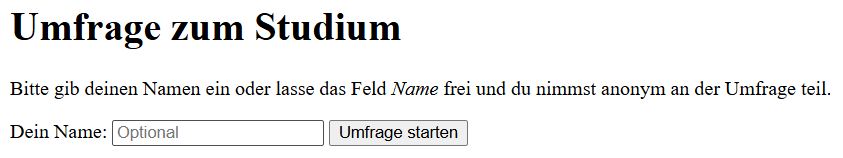
\includegraphics[width=0.9\textwidth]{./asset/image/Aufgabe3.png}
    \caption[Startseite \texttt{index.php} (\textit{Quelle: Eigene Darstellung})]
            {Startseite \texttt{index.php} (\textit{Quelle: Eigene Darstellung})\\ 
            \url{http://localhost/survey/index.php}}
    \label{fig:index}
\end{figure}

\section{Datei \texttt{survey.php}}

Die Datei \texttt{survey.php} empfängt den übergebenen Namen per \texttt{\$\_GET} und bereitet die Umfrage für den Teilnehmer vor. Sie stellt den Namen des Teilnehmers dar und zeigt vorbereitend die fünf Umfragefragen an.

\subsection{Vollständiger Quellcode}

\lstinputlisting[
    language=php, 
    caption={Umfrageseite \texttt{survey.php}}, 
    label={lst:survey-php}
]{asset/code/Aufgabe3II.tex}

\subsection{Erläuterung}

\subsubsection{Auslesen des GET-Parameters}

Der übergebene Name wird wie folgt aus der \acs{URL} ausgelesen:

\begin{lstlisting}[language=php]
$name = isset($_GET['name']) ? $_GET['name'] : '';
\end{lstlisting}

Die Funktion \texttt{isset()} prüft, ob der Parameter \texttt{name} überhaupt gesendet wurde. Falls nicht, wird ein leerer String als Fallback verwendet.

\subsubsection{Anonyme Teilnahme}

Wenn der Name leer ist oder nur aus Leerzeichen besteht, wird der Teilnehmer als \texttt{anonym} gekennzeichnet:

\begin{lstlisting}[language=php]
if (trim($name) === '') {
    $displayName = 'anonym';
    $userId = null;
}
\end{lstlisting}

\subsubsection{\acs{XSS}-Schutz}

Zur Sicherheit wird der Name vor der Ausgabe mit \texttt{htmlspecialchars()} kodiert:

\begin{lstlisting}[language=php]
$displayName = htmlspecialchars($name, ENT_QUOTES, 'UTF-8');
\end{lstlisting}

Dies verhindert Cross-Site-Scripting (\textit{\acs{XSS}})-Angriffe, bei denen ein Angreifer versuchen könnte, schädlichen JavaScript-Code über das Namensfeld einzuschleusen. Die Funktion wandelt folgende Zeichen in \acs{HTML}-Entities um:

\begin{table}[h]
\centering
\begin{tabular}{|c|c|}
\hline
\textbf{Zeichen} & \textbf{HTML-Entity} \\
\hline
\texttt{\&} & \texttt{\&amp;} \\
\texttt{"} & \texttt{\&quot;} \\
\texttt{'} & \texttt{\&\#039;} \\
\texttt{<} & \texttt{\&lt;} \\
\texttt{>} & \texttt{\&gt;} \\
\hline
\end{tabular}
\caption{Umwandlung von Sonderzeichen durch \texttt{htmlspecialchars()}}
\label{tab:htmlspecialchars}
\end{table}

\subsubsection{Weiterleitung der Daten}

Ein verstecktes Formularfeld (\textit{\texttt{hidden}}) speichert den Namen für die spätere Verarbeitung:

\begin{lstlisting}[language=html]
<input type="hidden" name="name" value="<?php echo htmlspecialchars($name, ENT_QUOTES, 'UTF-8'); ?>">
\end{lstlisting}

\section{Test der Namensübergabe}

Die Funktionalität der Namensübergabe wurde mit verschiedenen Eingaben getestet:

\subsection{Test 1: Name mit lateinischen Buchstaben}

\begin{figure}[h]
    \centering
    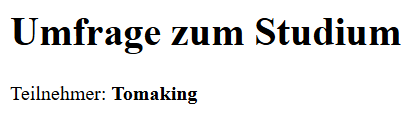
\includegraphics[width=0.5\textwidth]{./asset/image/Aufgabe3II.png}
    \caption[Umfrageseite \texttt{survey.php} (\textit{Quelle: Eigene Darstellung})]
            {Umfrageseite \texttt{survey.php} (\textit{Quelle: Eigene Darstellung})\\ 
            \url{http://localhost/survey/survey.php?name=Tomakin}}
    \label{fig:survey}
\end{figure}

\subsection{Test 2: Name mit Umlauten (\textit{\acs{URL}-kodiert})}

\begin{figure}[h]
    \centering
    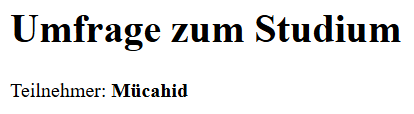
\includegraphics[width=0.5\textwidth]{./asset/image/Aufgabe3III.png}
    \caption[Umfrageseite \texttt{survey.php} (\textit{Umlaut}) (\textit{Quelle: Eigene Darstellung})]
            {Umfrageseite \texttt{survey.php} (\textit{Umlaut}) (\textit{Quelle: Eigene Darstellung})\\ 
            \url{http://localhost/survey/survey.php?name=M\%C3\%BCcahid}}
    \label{fig:surveyii}
\end{figure}

Der Umlaut \texttt{ü} wird korrekt aus der \acs{URL}-kodierten Form (\texttt{\%C3\%BC}) zurückkonvertiert und dargestellt.

\subsection{Test 3: Leeres Namensfeld (\textit{anonym})}

\begin{figure}[h]
    \centering
    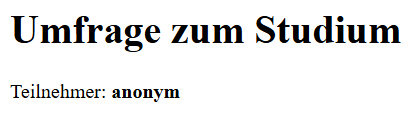
\includegraphics[width=0.5\textwidth]{./asset/image/Aufgabe3IV.png}
    \caption[Umfrageseite \texttt{survey.php} (\textit{Leer}) (\textit{Quelle: Eigene Darstellung})]
            {Umfrageseite \texttt{survey.php} (\textit{Leer}) (\textit{Quelle: Eigene Darstellung})\\ 
            \url{http://localhost/survey/survey.php?name=}}
    \label{fig:surveyiii}
\end{figure}

Bei leerem Parameter wird der Teilnehmer korrekt als \texttt{anonym} identifiziert.

\section{Zusammenfassung}

Die beiden Einstiegsseiten der Umfrageanwendung wurden erfolgreich implementiert:

\begin{itemize}
    \item \texttt{index.php} nimmt den Namen des Teilnehmers entgegen.
    \item Die Übergabe erfolgt per GET an \texttt{survey.php}.
    \item \texttt{survey.php} empfängt den Namen, bereitet ihn für die Anzeige auf und kennzeichnet leere Eingaben als anonym.
    \item Die Ausgabe wurde mit verschiedenen Eingaben (\textit{lateinische Buchstaben, Umlaute, leer}) erfolgreich getestet.
    \item Die Seiten sind gegen \acs{XSS}-Angriffe geschützt.
\end{itemize}

Die Dateien liegen unter folgenden Pfaden:

\begin{forest}
    for tree={
        font=\ttfamily,
        grow'=0,
        child anchor=west,
        parent anchor=south,
        anchor=west,
        calign=first,
        edge path={
            \noexpand\path [draw, \forestoption{edge}] (!u.south west) +(10pt,0) |- node[fill,inner sep=1.5pt] {} (.child anchor)\forestoption{edge label};
        },
        before typesetting nodes={
            if n=1{
                insert before={[,phantom,calign with current]}
            }{}
        },
        fit=band,
        before computing xy={l=22pt},
    }
    [\textbf{C:\textbackslash xampp\textbackslash htdocs\textbackslash survey}
        [\textbf{index.php}]
        [\textbf{survey.php}]
    ]
\end{forest}

Die Grundstruktur für die Umfrage ist damit geschaffen.

% ==============================================================================
% =================================== Aufgabe 3 ================================
% ==============================================================================